\documentclass[12pt, a4paper]{scrreprt}

\usepackage{amssymb}
\usepackage{graphicx}
\usepackage{listings}
\usepackage{xcolor}
\usepackage{hyperref}
\usepackage[table]{xcolor}

\hypersetup{
	colorlinks=true,
	linkcolor=blue,
	urlcolor=blue,
	citecolor=blue
}

\definecolor{codebg}{RGB}{40,44,52}        
\definecolor{codeframe}{RGB}{60,63,65}     
\definecolor{keywordcolor}{RGB}{198,120,221} 
\definecolor{commentcolor}{RGB}{128,128,128} 
\definecolor{stringcolor}{RGB}{255,208,0}    
\definecolor{identifiercolor}{RGB}{97,175,239}
\definecolor{numbercolor}{RGB}{209,154,102}   

\definecolor{ms1}{RGB}{230,240,255} 
\definecolor{ms2}{RGB}{235,225,255} 
\definecolor{ms3}{RGB}{255,230,230} 

\lstdefinestyle{IntelliJPurple}{
	backgroundcolor=\color{codebg},
	frame=single,
	framerule=1pt,
	framesep=3pt,        
	basicstyle=\ttfamily\small\color{white},
	keywordstyle=\color{keywordcolor}\bfseries,
	commentstyle=\color{commentcolor}\itshape,
	stringstyle=\color{stringcolor},
	identifierstyle=\color{identifiercolor},
	numberstyle=\tiny\color{gray},
	numbers=left,
	stepnumber=1,
	numbersep=5pt,
	showstringspaces=false,
	breaklines=true,
	tabsize=4,
	captionpos=b,
	xleftmargin=0pt,    
	numbersep=5pt,       
}

\lstdefinelanguage{JavaScript}{
	keywords={var, let, const, function, if, else, return},
	sensitive=true,
	comment=[l]{//},
	morecomment=[s]{/*}{*/},
	morestring=[b]"
}

\title{Softwarearchitektur Projektarbeit}
\subtitle{Projektplan}
\author{Gruppe 1 - Team 2\\Ayleen Edenhauser, Matteo Volperino,\\Jakob Oberhofer, Leonid Georg Mikhailovic Stommel (Ljonja)}
\date{WS 2025/26}

\renewcommand{\familydefault}{\sfdefault}

\titlehead{
	\raggedright
	\vspace*{3cm}
	
\includegraphics[width=0.6\textwidth]{logo.jpg}
}

\begin{document}
	
	\maketitle
		
	\tableofcontents
	
	\chapter{Einleitung}
	
	Dieser Projektplan beschreibt die geplante Umsetzung unseres Projekts. In der Einleitung wird zunächst die grundlegende Nutzung des Webshops erläutert. Die folgenden Kapitel behandeln die verschiedenen \textit{Aspekte des Projekts} und zeigen auf, wie diese \textit{miteinander interagieren}. Ziel dieses Dokuments ist es, einen \textbf{strukturierten und nachvollziehbaren Projektplan} zu erstellen, der als Orientierung für die weitere Projektarbeit dient.

		\section{Workflow}
		
		Ein User besucht den Webshop und landet auf der Homepage, welche eine Gallery View aller Produkte ist. Der User sieht zu jedem Produkt:
		\begin{itemize}
			\item Das \textbf{Produktbild} (dient als Button)
			\item Die \textbf{Produktkategorie} 
			\item Den \textbf{Preis}
			\item Falls ein \textbf{Rabatt} vorhanden ist:
				\begin{itemize}
					\item Den rabattierten Preis (in rot)
					\item Daneben den ursprünglichen Preis
					\item Die Kategorie "Sale"
				\end{itemize}
			\item Die Kategorie \textbf{"Out of stock"} falls ausverkauft
		\end{itemize}
		
		Der User hat die Möglichkeit Produkte nach folgenden Kriterien zu \textbf{filtern und sortieren}:
		\begin{itemize}
			\item Produktkategorie
			\item Preis unter 10€, 25€ oder 50€
			\item Sortiert nach Preis aufsteigend oder absteigend
			\item Alphabetisch sortiert nach Produktnamen
		\end{itemize}
		
		Der User interessiert sich für ein Produkt und klickt auf ein Produktbild, er landet auf der Seite zu diesem Produkt. Dort hat er die Optionen das \textbf{Produkt in den Warenkorb} zu legen oder es zu \textbf{abonnieren}. 
		
		Hier sieht der User außerdem die Produktbeschreibung und am Ende der Seite alle \textbf{Bewertungen} in einem List View. Hier ist \textbf{Sortierung und Filterung} nach folgenden Kriterien möglich:
		\begin{itemize}
			\item Vergebene Sterne
			\item Sortiert nach Sternen aufsteigend oder absteigend
		\end{itemize}
		Angemeldet User können \textbf{Bewertungen hinterlassen}. Jede Bewertung besteht aus:
		\begin{itemize}
			\item \textbf{1-5 Sternen}
			\item Einem \textbf{Kommentar}
		\end{itemize}
		
		Möchte der User ein Produkt in den Warenkorb legen, kann er das auch \textbf{ohne Konto}. Er \textbf{wählt die Stückzahl} in Form von einem "-/+"-Button aus und drückt auf "Add to cart". Besitzt das Produkt die Kategorie "Out of stock", bekommt der User einen \textbf{Fehler "Cannot add product to cart, out of stock."}.
		
		Möchte der User ein Produkt \textbf{abonnieren}, wird er aufgefordert sich \textbf{anzumelden oder zu registrieren}. Ab jetzt wird der User über \textbf{Preisveränderungen} und \textbf{Restocks} informiert. Der \textbf{"Subscribe"-Button} wird das Icon zu einem Haken geändert, wird er nochmal geklickt sind die \textbf{Benachrichtigungen wieder deabonniert}.
		
		Der User wählt eine Stückzahl und klickt "Add to cart", im \textbf{Header} erscheint eine "1" neben dem \textbf{Warenkorb-Symbol}. Er klickt auf das Symbol und kommt auf die Warenkorb-Seite. Dort sieht der User in einem List View alle Produkte aufgezählt:
		\begin{itemize}
			\item \textbf{Produktname}
			\item \textbf{Preis pro Stück} zum Zeitpunkt des Hinzufügens
			\item \textbf{Stückzahl}
			\item \textbf{Gesamtpreis pro Produkt}
			\item Am Ende den \textbf{Gesamtpreis der Bestellung}
		\end{itemize}
		
		Auch hier besteht die Option nach den oben genannten Kriterien zu filtern und zu sortieren.
		In jeder Zeile befindet sich ein weiterer "-/+"-Button zum \textbf{anpassen der Stückzahl} und ein \textbf{"Remove from cart"-Button}.
		
		Der User passt alles zu seiner Zufriedenheit an und klickt auf \textbf{"Buy"}. Spätestens hier wird der User zur Registrierung oder Anmeldung aufgefordert. Eine \textbf{Bestellung} wird erstellt und in der \textbf{Bestellhistorie} des Users gespeichert. 
		Die Bestellhistorie ist ein List View bestehend aus:
		\begin{itemize}
			\item \textbf{Bestellnummer}
			\item \textbf{Gesamtpreis}
			\item \textbf{Datum der Bestellung}
		\end{itemize}
		Auch diese Liste ist \textbf{sortier- und filterbar}:
		\begin{itemize}
			\item Datum der Bestellung vor einer Woche, Monat oder Jahr
			\item Aufsteigend oder absteigend nach Datum sortiert 
		\end{itemize}
		
		Klickt der User auf eine Bestellung, sieht er die \textbf{Rechnung}, eine einfache Auflistung ähnlich zu der im Warenkorb, nur nicht durch den User veränderbar und sie inkludiert die \textbf{User-Details}:
		\begin{itemize}
			\item \textbf{Vor- und Nachname}
			\item \textbf{Adresse}
		\end{itemize}
		
		Zusätzlich zu diesen Funktionen können User mit der \textbf{Rolle}:
		\begin{itemize}
			\item \textbf{Manager}
				\begin{itemize}
					\item Auf der Produktseite auf "Edit" klicken und Produktdetails anpassen
					\item Im Header auf "Add new product" klicken und ein neues Produkt hochladen
				\end{itemize}
			\item \textbf{Admin}
				\begin{itemize}
					\item Auf der Produktseite auf "Edit" klicken und Produktdetails anpassen
					\item Im Header auf "Add new product" klicken und ein neues Produkt hochladen
					\item User-Konten verwalten
				\end{itemize}
		\end{itemize}
		
			\subsection{Sequenzdiagramm}
			
			\textbf{ToDo}
			
			\subsection{Fachliches Klassendiagramm}
			
			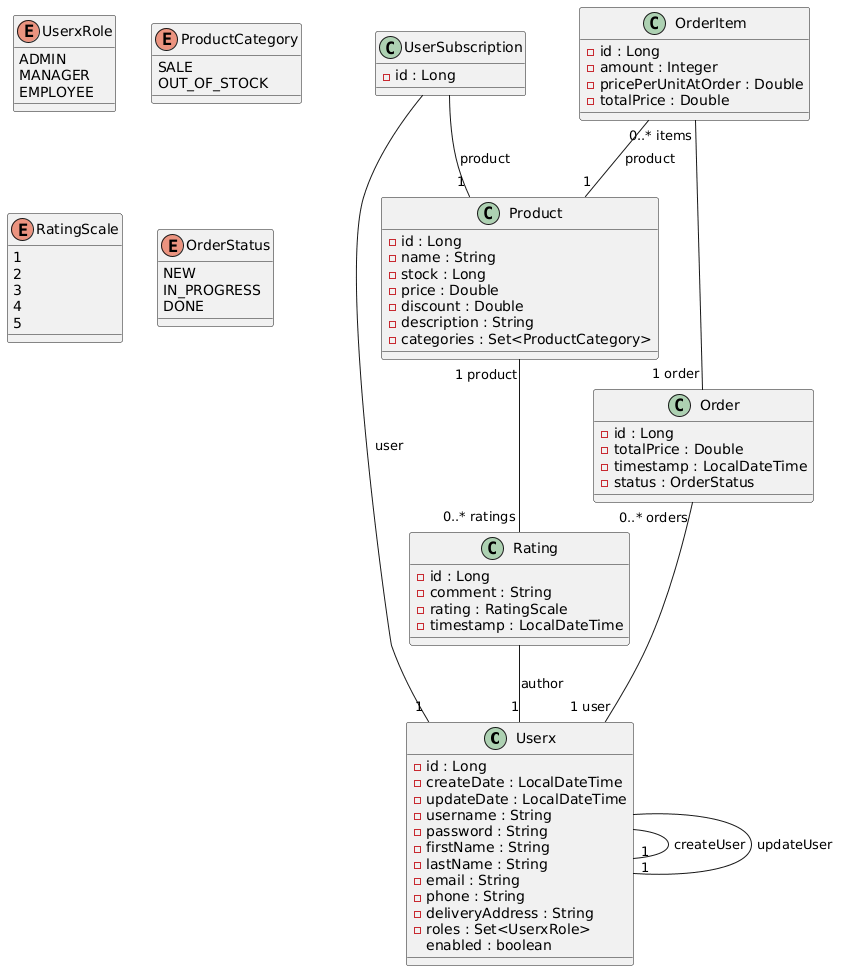
\includegraphics[width=1\textwidth]{fachliches_uml.png}
			
		\section{Meilensteine}
			
			\subsection*{Meilenstein 1 - Backend und Tests}
			
			Das Ziel von Meilenstein 1 ist es, die \textbf{Basisfunktionen} für die uns zugewiesenen Features zu implementieren, vorerst nur im Backend. Anschließend sollen UnitTests für das Backend geschrieben werden. Für den Warenkorb wird hier die Implementation im Frontend verlangt, da er nur dort existiert.
			
			\textbf{Deadline} ist der 31.12.2026.
			
			\subsection*{Meilenstein 2 - Frontend und Feature-Erweiterung}
			
			Das Ziel von Meilenstein 2 ist es, das Frontend für die uns zugewiesenen Features zu implementieren und gemeinsam die User-Verwaltung und das Abonnements-System auszuarbeiten.
			
			\textbf{Deadline} ist der 12.01.2026.
			
			\subsection*{Meilenstein 3 - Fertiges Produkt}
			
			Das Ziel von Meilenstein 3 ist es, das \textbf{Projekt fertig} zu stellen. Bis hierhin sollen nurnoch Inkonsistenzen behandelt, Fehler behoben und gemeinsam die Fehlerbehandlung ausgearbeitet werden.
			
			Die \textbf{Abgabe} erfolgt dann am 02.02.2026.
			
			\textbf{Deadline} ist der 31.01.2026.
			
		\section{Issues}
		
		Allgemein wird wie folgt nach Features aufgeteilt:
		\begin{itemize}
			\item \textbf{Produkte} (ohne Abonnements): Ljonja
			\item \textbf{Bewertungen}: Matteo
			\item \textbf{Bestellungen}: Jakob
			\item \textbf{Warenkorb}: Ayleen
			\item \textbf{User}, \textbf{Abonnements} und \textbf{Fehlerbehandlung}: Gruppenarbeit 
		\end{itemize}
		
		\begin{table}[h]
			\centering
			\caption{Zu erstellende Issues}
			\label{tab:example}
			\begin{tabular}{|p{2.5cm}|p{2.5cm}|p{5cm}|p{2.5cm}|p{2.5cm}|}
				\hline
				\textbf{Issue} & \textbf{Feature} & \textbf{Beschreibung} & \textbf{Zugewiesen} & \textbf{Deadline} \\ \hline
				
				\rowcolor{ms1}
				Implement feature in backend & Produkte & Implement the backend for the products and test it, ratings and subscribtions excluded & Ljonja & Meilenstein 1\\ \hline
				
				\rowcolor{ms1}
				Implement feature in backend& Bewertungen & Implement the backend for the ratings and test it & Matteo & Meilenstein 1\\ \hline
				
				\rowcolor{ms1}
				Implement feature & Warenkorb & Implement the  shopping cart and test it, only exists in frontend  & Ayleen & Meilenstein 1\\ \hline
				
				\rowcolor{ms1}
				Implement feature in backend& Bestellungen & Implement the backend for the orders and test it & Jakob & Meilenstein 1\\ \hline
				
				\rowcolor{ms2}
				Implement feature in frontend & Produkte & Implement the frontend for the products, ratings and subscribtions excluded & Ljonja & Meilenstein 2\\ \hline
				
				\rowcolor{ms2}
				Implement feature in frontend& Bewertungen & Implement the frontend for the ratings  & Matteo & Meilenstein 2\\ \hline
				
				\rowcolor{ms2}
				Implement feature in frontend& Bestellungen & Implement the frontend for the orders & Jakob & Meilenstein 2\\ \hline
				
				\rowcolor{ms2}
				Implement managers & User & Implement all remaining user features for managers and test them& Alle (oder Ayleen?) & Meilenstein 2\\ \hline
				
				\rowcolor{ms2}
				Implement subscribtion system & Produkte & Implement subscribtion logic and test it & Alle (oder Ayleen?)  & Meilenstein 2\\ \hline
				
				\rowcolor{ms3}
				Error handling & Fehler & Collect all existing errors and implement error handling and test it & Alle & Meilenstein 3\\ \hline
				
				\rowcolor{ms3}
				Bug fixes & - & Finalise the project & Alle & Meilenstein 3\\ \hline
			\end{tabular}
		\end{table}
		
	
	\chapter{User}
	
	Registrierte User sind eine \textbf{Datenbankentität}. Der Großteil des User-Managements ist bereits implementiert. 
	
		\section{Attribute}
		
		Jeder User hat:
		\begin{itemize}
			\item ID
			\item Vor- und Nachname
			\item Email
			\item Telefonnummer
			\item Username
			\item Einen Boolean-Wert \texttt{enabled}
			\item Einen \texttt{createUser} und \texttt{createDate}
			\item Einen \texttt{updateUser} und \texttt{updateDate}
			\item Eine Sammlung von Bestellungen, Bewertungenm Rollen und Abonnements
		\end{itemize}
	
			\subsection{Rollen}
			
			Startet man die Web Applikation ist man vorerst ein \textbf{Besucher}, also ein unangemeldeter Nutzer, der nur die Option hat, seinen Warenkorb zu befüllen. Bei jeder anderen Funktion wird der zuerst zur Seite "Log-in or register" gebracht.
			
			\textbf{Angemeldete User} haben eine oder mehrere Rollen.
			
			Normale \textbf{User} können bestellen, die Bestellhistorie einsehen, Produkte abonnieren und Bewertungen hinterlassen.
			
			\textbf{Manager} haben zusätzlich auf der Seite jedes Produkts einen "Edit"-Button, ähnlich zu dem im bereits bestehenden User-Management-System. Ihnen erscheint im Header ein "Add new product"-Button.
			
			\textbf{Admins} können alles was Manager und User können, und haben Zugriff auf die User-Verwaltung.
		
		
		\section{Involvierte Klassen}
		
		\begin{itemize}
			\item \texttt{Userx}: Die Datenbankentität 
			\item \texttt{UserxRole}: Ein Enum zu den Rollen
			\begin{itemize}
				\item \texttt{USER}
				\item \texttt{MANAGER}
				\item \texttt{ADMIN}
			\end{itemize}
			\item \texttt{UserxRepository}: Kommuniziert direkt mit der Datenbank
			\item \texttt{UserxService}: Stellt zusätzliche Datenbankfunktionen zur Verfügung
			\item \texttt{AuthenticatedUserService}: stellt das aktuell authentifizierte User-Objekt bereit
			\item \texttt{AuthenticationService}: authentifiziert Benutzer und erzeugt nach erfolgreicher Anmeldung ein JWT zur weiteren Autorisierung
			\item \texttt{UserxMapper}: Konversion zwischen Userx und UserxDTO
			\item \texttt{UserxCreateMapper}: Konversion zwischen Userx und UserxCreateDTO
			\item \texttt{UserxDTO}: Datentransferobjekt zur User-Verwaltung
			\item \texttt{UserxCreateDTO}: Datentransferobjekt zur User-Erstellung
			\item \texttt{LoginResponseDTO}: kapselt das nach erfolgreicher Authentifizierung erzeugte JWT
			\item \texttt{LoginRequestDTO}: Datentransferobjekt zur User-Authentifizierung
			\item \texttt{UserxController}, \texttt{AuthenticationController}, \texttt{ManagerController}\\und \texttt{AdminController}: Weisen HTTP Anfragen Methoden zu
		\end{itemize}

	\chapter{Produkte}
	
	Produkte sind eine \textbf{Datenbankentität}.
	
		\section{Attribute}
		
		Jedes Produkt hat:
		\begin{itemize}
			\item ID
			\item Name
			\item Preis
			\item Rabatt
			\item Bestand
			\item Produktbild
			\item Beschreibung
			\item Eine Sammlung von Bewertungen und Kategorien
		\end{itemize}
	
			\subsection{Bewertungen}
			
			Auch Bewertungen sind eine \textbf{Datenbankentität}.
			
				\subsubsection{Attribute}
				
				Jede Bewertung hat:
				\begin{itemize}
					\item ID
					\item Autor
					\item Bewertung in \texttt{RatingScale}
					\item Timestamp
					\item Produkt
				\end{itemize}
		
		\section{Abonnements}
		
		Abonnements sind mithilfe vom \href{https://springframework.guru/gang-of-four-design-patterns/observer-pattern/}{Spring \textbf{Observer}} umgesetzt, oft auch \textbf{"Publisher-Subscriber"} genannt.
			
		Bei einem Abonnement wird der User \textbf{über Restocks und Rabatte informiert}. Wir definieren also 2 \textbf{Events}, welche beide von \texttt{ApplicationEvent} erben:
		\begin{itemize}
			\item \texttt{ProductRestockEvent}
			\item \texttt{ProductSaleEvent}
		\end{itemize}
		Diese sind wie folgt aufgebaut:
		
		\begin{lstlisting}[style=IntelliJPurple, language=Java]
public class ProductRestockEvent extends ApplicationEvent {
	private final Long productId;
	
	public ProductRestockEvent(Object source, Long productId) {
		super(source);
		this.productId = productId;
	}
	
	public Long getProductId() {
		return productId;
	}
}
		\end{lstlisting}
		
		Zudem brauchen wird einen \textbf{Publisher}, der über Events informiert. Der \texttt{ApplicationEventPublisher} existiert bereits in Spring und muss nurnoch in einen Service injiziert werden. Das sieht dann ungefähr wie folgt aus:
		
		\begin{lstlisting}[style=IntelliJPurple, language=Java]
@Service
public class ProductService {
	@Autowired
	private ApplicationEventPublisher publisher;
	
	public void restockProduct(Long productId) {
		// ...
		publisher.publishEvent(new ProductRestockEvent(this, productId));
	}
}
		\end{lstlisting}
		
		Zuletzt benötigen wir noch einen Subscriber.

		\begin{lstlisting}[style=IntelliJPurple, language=Java]
@Component
public class ProductEventListener {
	@EventListener
	public void handleRestock(ProductRestockEvent event) {
		// Notify user
	}
	
	@EventListener
	public void handleSale(ProductSaleEvent event) {
		// Notify user
	}
}
		\end{lstlisting}
		
			\subsection{Ablauf}
		
			Ein Abonnement abzuschließen erfolgt mit dieser Implementation so:
			\begin{itemize}
				\item[1.] Der User klickt im Frontend auf der Produktseite auf "Subscribe".
				\item[2.] Das Frontend sendet eine Anfrage an den Backend-Endpoint, der den User für das Produkt registriert.
				\item[3.] Der Backend-Service speichert die Abonnement-Relation in der Datenbank.
				\item[4.] Wenn ein Event wie \texttt{ProductRestockEvent} oder \texttt{ProductSaleEvent} ausgelöst wird, empfängt der \texttt{ProductEventListener} dieses Event.
				\item[5.] Der Listener filtert die User, die das Produkt abonniert haben, und benachrichtigt sie über die gewünschte Methode.
			\end{itemize}

	
		\section{Involvierte Klassen}
		
		\begin{itemize}
			\item \texttt{Product}, \texttt{Rating} und \texttt{UserSubscription}: Die Datenbankentitäten
			\item \texttt{ProductCategory}: Ein Enum zu den Kategorien
			\begin{itemize}
				\item \texttt{SALE}
				\item \texttt{OUT\_OF\_STOCK}			
				\item Weitere Kategorien je nach Produkttyp
			\end{itemize}
			\item \texttt{RatingScale}: Ein Enum zu den vergebenen Sternen
			\item \texttt{ProductRepository}, \texttt{RatingRepository} und \texttt{UserSubscriptionRepository}: Kommuniziert direkt mit der Datenbank
			\item \texttt{ProductService},  \texttt{RatingService} und \texttt{UserSubscriptionService}:\\ Stellt zusätzliche Datenbankfunktionen zur Verfügung
			\item \texttt{ProductController} und \texttt{SubscriptionController}: Weisen HTTP Anfragen Methoden zu
			\item \texttt{ProductMapper}: Konversion zwischen \texttt{Product} und \texttt{ProductDTO}
			\item \texttt{ProductDTO}: Datentransferobjekt für Frontend
			\item \texttt{ProductCreateDTO}: Datentransferobjekt zur Produkterstellung
			\item \texttt{SubscriptionRequestDTO}: Datentransferobjekt zum Abschließen eines Abonnements
			\item \texttt{ProductEventListener}: Versendet Benachrichtigungen
			\item \texttt{ProductRestockEvent} und \texttt{ProductSaleEvent}: Mögliche Benachrichtigungen
		\end{itemize}
		
	\chapter{Warenkorb}
	
	Der Warenkorb ist keine Datenbankentität sondern wird per Local Storage \textbf{im Browser gespeichert}.
	
	Beim Hinzufügen eines Produkts wird der aktuelle \textbf{Warenkorb geladen}, das \textbf{Produkt hinzugefügt} oder die \textbf{Stückzahl angepasst}, und der \textbf{Warenkorb wieder gespeichert}. Produkte können entfernt oder die Stückzahl angepasst werden. Beim Laden der Warenkorb-Seite wird der gespeicherte Warenkorb ausgelesen und angezeigt.
	
	Das soll ungefähr so funktionieren:
	
			\begin{lstlisting}[style=IntelliJPurple, language=JavaScript]
// Add product to cart
function addToCart(productId, quantity) {
	let cart = JSON.parse(localStorage.getItem('cart')) || [];
	const existing = cart.find(item => item.id === productId);
	if (existing) {
		existing.quantity += quantity;
	} else {
		cart.push({ id: productId, quantity });
	}
	localStorage.setItem('cart', JSON.stringify(cart));
}

// Read cart
function getCart() {
	return JSON.parse(localStorage.getItem('cart')) || [];
}

// Remove product
function removeFromCart(productId) {
	let cart = JSON.parse(localStorage.getItem('cart')) || [];
	cart = cart.filter(item => item.id !== productId);
	localStorage.setItem('cart', JSON.stringify(cart));
}
	\end{lstlisting}
	
	\section{Attribute}
	
	Den Warenkorb an sich gibt es nicht, nur das DTO. Jedes davon hat:
	\begin{itemize}
		\item Eine Sammlung an \texttt{CartItemDTO}
	\end{itemize}
	
	Jedes \texttt{CartItemDTO} hat:
	\begin{itemize}
		\item Produkt-ID
		\item Produktname
		\item Preis pro Stück
		\item Stückzahl
	\end{itemize}
	
	\section{Involvierte Klassen}
	
	\begin{itemize}
		\item \texttt{CartDTO}: Speichert Produkte und deren Stückzahl 
		\item \texttt{CartItemDTO}: Datentransferobjekt für Produkte im Warenkorb
	\end{itemize}
	
	\chapter{Bestellungen}
	
	Bestellungen sind \textbf{Datenbankentitäten} und für die \textbf{Zahlungsabwicklung} verantwortlich. User haben Zugriff auf ihre Bestellhistorie.
	
		\section{Attribute}
		
		Jede Bestellung hat:
		\begin{itemize}
			\item ID
			\item Gesamtpreis
			\item Timestamp
			\item Status
			\item Den dazugehörigen User
			\item Eine Sammlung von \texttt{OrderItem}
		\end{itemize}
		
		Jedes \texttt{OrderItem} hat:
		\begin{itemize}
			\item Produkt-ID
			\item Name
			\item Preis pro Stück zum Bestellzeitpunkt
			\item Stückzahl
			\item Gesamtpreis
		\end{itemize}
		
			\subsection{Status}
			
			Der Status einer Bestellung \textbf{verändert sich automatisch}. Während die Bestellung erstellt wird ist sie \texttt{NEW}. Beginnt man die Zahlungsabwicklung, wird der Status auf \texttt{IN\_PROGRESS} gestellt. Sobald die Rechnung per Email "versendet" wurde und in der Bestellhistorie einzusehen ist, ist sie unveränderbar und hat den Status \texttt{DONE}. 
		
			Der Status hat \textbf{keine weitere Funktion} und ist nur Aufgrund der Anforderungen implementiert.

		\section{Zahlungsabwicklung}
		
		Die Zahlungsabwicklung simuliert den Ablauf einer Bestellung. Es erfolgt \textbf{keine echte Transaktion}. Nach Abschluss wird der Bestellstatus entsprechend aktualisiert und eine Email "versendet".
		
		\section{Erstellung einer Bestellung}
		
		Eine Bestellung entsteht aus dem aktuellen Warenkorb des Users. Beim Abschließen des Bestellvorgangs werden die \textbf{Inhalte des Warenkorbs in eine neue \texttt{Order} mit entsprechenden \texttt{OrderItem} überführt}. Anschließend wird der Warenkorb geleert.
		
		
		\section{Involvierte Klassen}
		
		\begin{itemize}
			\item \texttt{Order} und \texttt{OrderItem}: Datenbankentitäten
			\item \texttt{OrderRepository}: Kommuniziert direkt mit der Datenbank
			\item \texttt{OrderService}: Stellt zusätzliche Datenbankfunktionen zur Verfügung
			\item \texttt{OrderStatus}: Ein Enum zum Bestellstatus
			\begin{itemize}
				\item \texttt{NEW}
				\item \texttt{IN\_PROGRESS}
				\item \texttt{DONE}
			\end{itemize}
			\item \texttt{OrderMapper}: Konversion zwischen \texttt{Order} und \texttt{OrderDTO}
			\item \texttt{OrderDTO}: Datentransferobjekt für Frontend
			\item \texttt{OrderController}: Weist HTTP Anfragen Methoden zu
		\end{itemize}
		
	\chapter{Fehlerbehandlung}
	
\end{document}